\documentclass[utf8x, handout]{beamer}
%\documentclass[handout,utf8x]{beamer}

\usepackage{pgf,tikz}
\usetikzlibrary{arrows}

%% pour franciser les noms definitin, theorem, proof, example
\uselanguage{French}
\languagepath{French}

%% style de beamer
\setbeamertemplate{background canvas}[vertical shading][top=blue!25,middle=white,midpoint=0.75]
\usecolortheme{default}
\useinnertheme{default}
\usefonttheme{structurebold}
\useoutertheme{smoothbars}
\setbeamertemplate{frametitle}[default][center]
\setbeamertemplate{navigation symbols}{} %% pour enlever les symboles de navigation
%% fin style

%\author{Vincent Deveaux}
\title{Analyse Fonctionnelle}
\author{TS-ISN}
\institute{Lycée Monge, Chambéry}
\date{2018}


\newcommand{\AFfun}[3]{\tiny \begin{tabular}{lll} #1 \\ \hline IN : #2 \\ OUT : #3 \\ \end{tabular}}


\begin{document}

%
%%%
\begin{frame}[plain]
    \titlepage

    \begin{center}
      
\includegraphics[width=5cm]{logo-monge.png}
    \end{center}
\end{frame}
%%%
%


%
%%%
\begin{frame}
  \frametitle{Qu'est-ce que c'est ?}
  \begin{itemize}
  \item<+-> Un schéma simple montrant les dépendances entre les fonctions.
    \bigskip
  \item<+-> Une signature claire pour chaque fonction (son nom, ses entrées, ses sorties et leurs types).
    \bigskip
  \item<+-> Des flèches pour matérialiser qui utilise qui.
  \end{itemize}
\end{frame}
%%%
%


%
%%%
\begin{frame}
  \frametitle{Ça ressemble à quoi ?}
  Calcul de moyenne : on demande une série de note et on affiche leur moyenne.
  \uncover<2>{
    \begin{center}
      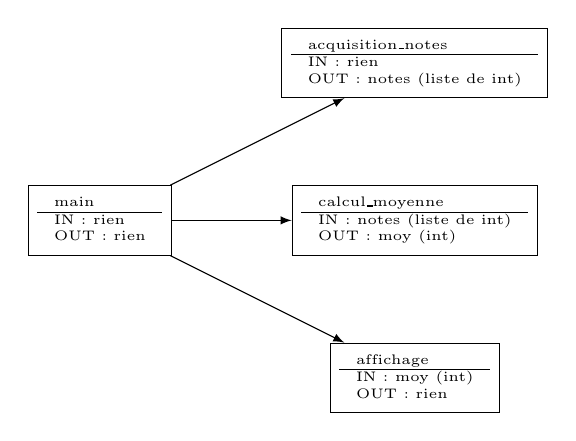
\begin{tikzpicture}
        \node[draw] (Prin) at (0,0) {\AFfun{main}{rien}{rien}};
        \node[draw] (Dema) at (4,2) {\AFfun{acquisition\_notes}{rien}{notes (liste de int)}};
        \node[draw] (Calc) at (4,0) {\AFfun{calcul\_moyenne}{notes (liste de int)}{moy (int)}};
        \node[draw] (Affi) at (4,-2) {\AFfun{affichage}{moy (int)}{rien}};
        \draw[->,>=latex] (Prin) edge (Dema) edge (Calc) edge (Affi);
      \end{tikzpicture}
    \end{center}
  }
\end{frame}
%%%
%


%
%%%
\begin{frame}
  \frametitle{Pour quoi faire ?}
  \begin{itemize}
  \item<+-> Refléchir à la logique du programme AVANT de taper du code.
    \bigskip
  \item<+-> Structurer ses idées (et donc sa pensée).
    \bigskip
  \item<+-> Décomposer les points délicats à programmer (diviser pour mieux régner).
  \end{itemize}
\end{frame}
%%%
%




%
%%%
\begin{frame}
  \frametitle{Les bonnes pratiques}
  \begin{itemize}
  \item<+-> Une fonction ou un bloc principal (main).
  \item<+-> Des noms de fonction explicites.
  \item<+-> Une fonction = peu d'actions.
  \item<+-> Séparer \dots
    \begin{itemize}
    \item<+-> la gestion des données,
    \item<+-> l'interaction homme-machine,
    \item<+-> la logique du programme.
    \end{itemize}
  \end{itemize}
\end{frame}
%%%
%




%
%%%
\begin{frame}
  \frametitle{A vous de jouer !}
  \begin{itemize}
  \item<+-> Deux équipes.
    \bigskip
  \item<+-> Analyse fonctionnelle de la gestion du jeu du morpion.
    \bigskip
  \item<+-> Comparaison des approches des deux camps.
  \end{itemize}
\end{frame}
%%%
%


%
%%%
\begin{frame}
  \frametitle{GO !!}
  Calcul de moyenne
  \begin{center}
    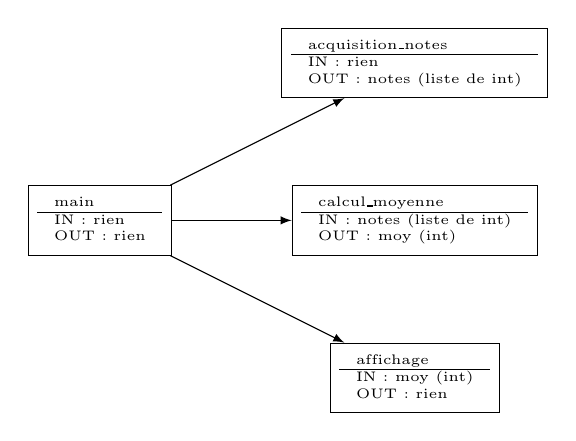
\begin{tikzpicture}
      \node[draw] (Prin) at (0,0) {\AFfun{main}{rien}{rien}};
      \node[draw] (Dema) at (4,2) {\AFfun{acquisition\_notes}{rien}{notes (liste de int)}};
      \node[draw] (Calc) at (4,0) {\AFfun{calcul\_moyenne}{notes (liste de int)}{moy (int)}};
      \node[draw] (Affi) at (4,-2) {\AFfun{affichage}{moy (int)}{rien}};
      \draw[->,>=latex] (Prin) edge (Dema) edge (Calc) edge (Affi);
    \end{tikzpicture}
  \end{center}
\end{frame}
%%%
%



\end{document}
